%~~~~~~~~~~~~~~~~%
\section{TownWorkの旅}
%~~~~~~~~~~~~~~~~%
%===========================%
\subsection{現在までに取得できた統計情報}
%===========================%
本章では各地方の就業率とバイトの募集の関係性を論じるための行脚についての報告を行う。
バイトの募集情報ソースにはタウンワークを採用し公平性を持たせた。
タウンワークが発行されている県と発行されていない県も存在し、発行されていない県については
タウンワークと同等の公平性・正確性を持っている雑誌を参考とした。
特に岩手県は「求人ジャーナル」を採用した。
以下に現在(2018年3月27日)までに取得できた統計情報を示す。
今後はさらに出張を重ね、統計量を増やし統計誤差は削減されると期待される。

\begin{figure}[htbp]
\vspace{-10mm}
    \centering
  \begin{minipage}{0.4\linewidth}
    \centering
    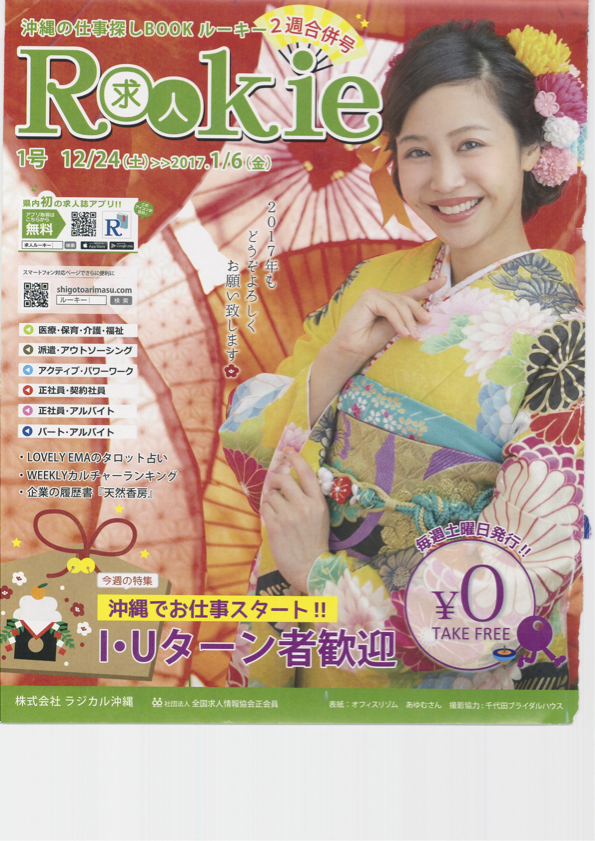
\includegraphics[scale=0.2]{tw}
  \end{minipage}
  \begin{minipage}{0.4\linewidth}
    \centering
    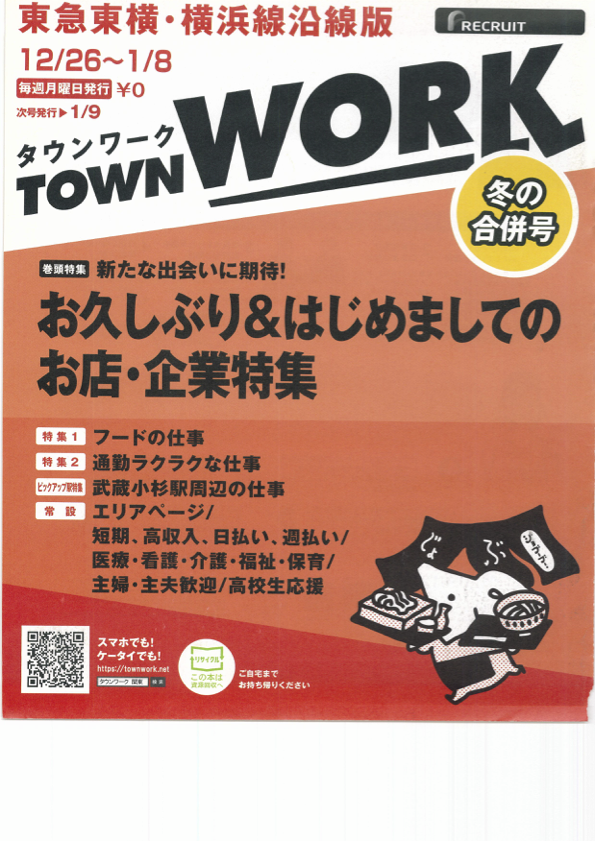
\includegraphics[scale=0.2]{tw1}
  \end{minipage}\\
  \begin{minipage}{0.4\linewidth}
    \centering
    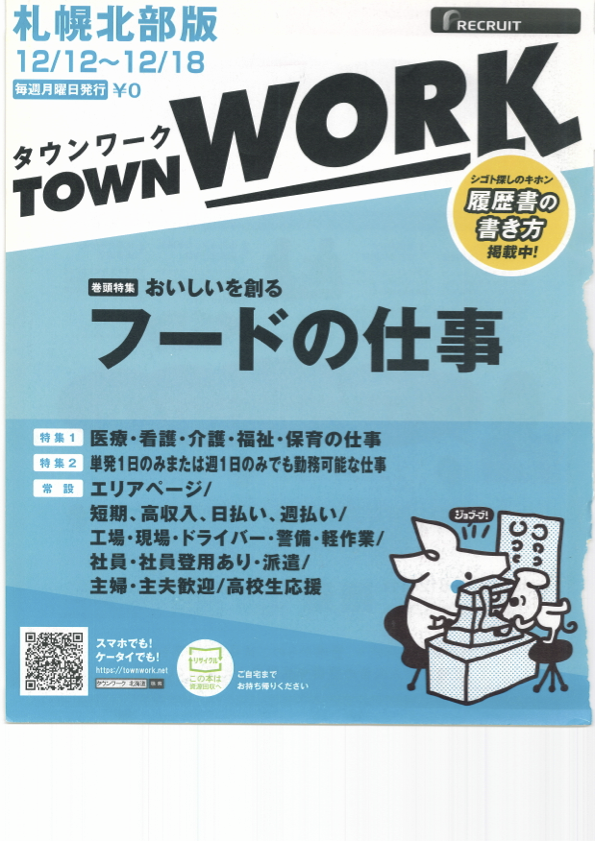
\includegraphics[scale=0.2]{tw2}
  \end{minipage}
  \begin{minipage}{0.4\linewidth}
    \centering
    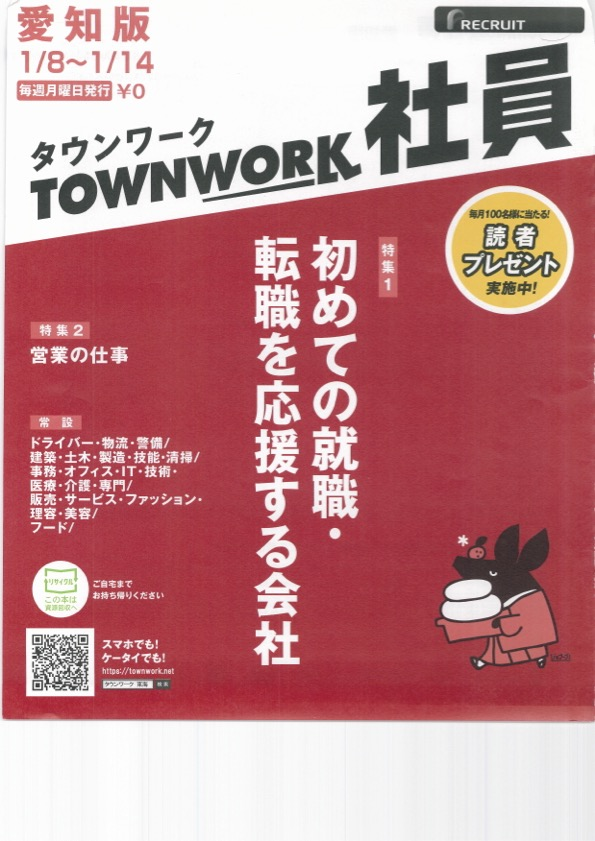
\includegraphics[scale=0.2]{tw3}
  \end{minipage}
  \begin{minipage}{0.4\linewidth}
    \centering
    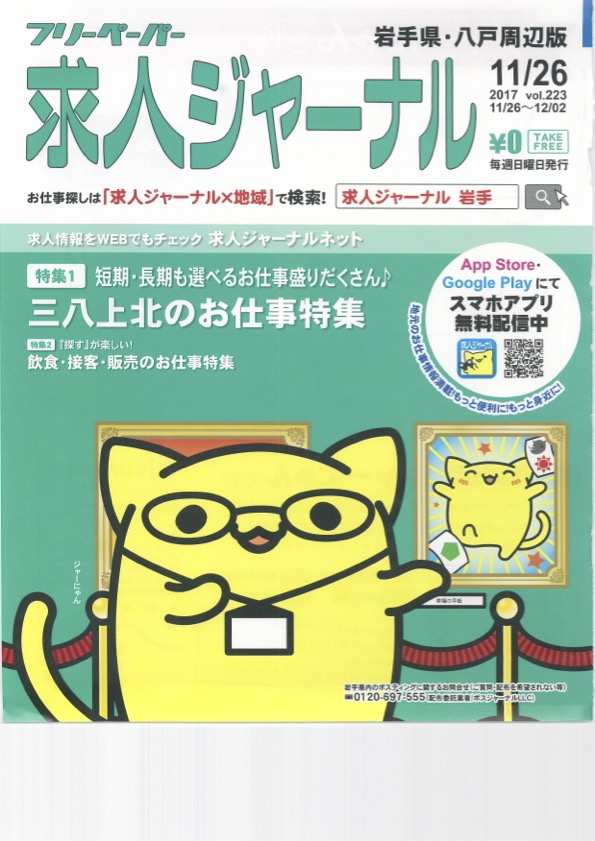
\includegraphics[scale=0.2]{tw4}
  \end{minipage}
  \begin{minipage}{0.4\linewidth}
    \centering
    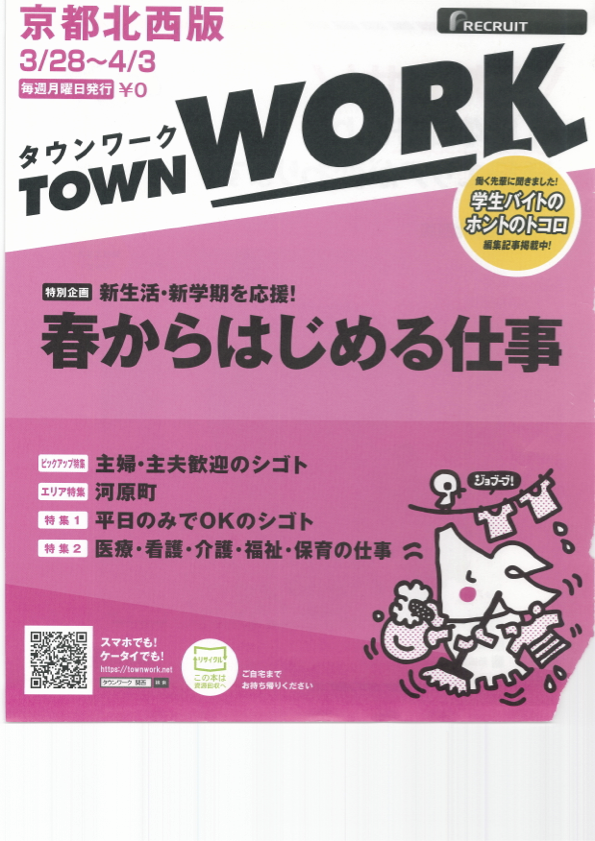
\includegraphics[scale=0.2]{tw5}
  \end{minipage}
  \caption{TownWorkの旅で手に入れた各地方の表紙一覧。}
  \label{CscDetaDphi-CSide}
\end{figure}

\newpage
\begin{figure}[htbp]
\vspace{-10mm}
    \centering
  \begin{minipage}{0.4\linewidth}
    \centering
    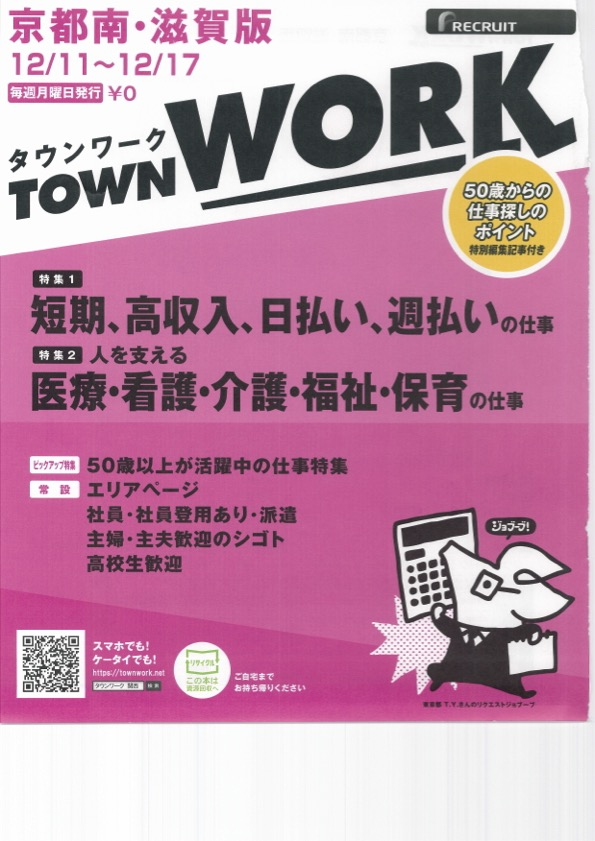
\includegraphics[scale=0.2]{tw6}
  \end{minipage}
  \begin{minipage}{0.4\linewidth}
    \centering
    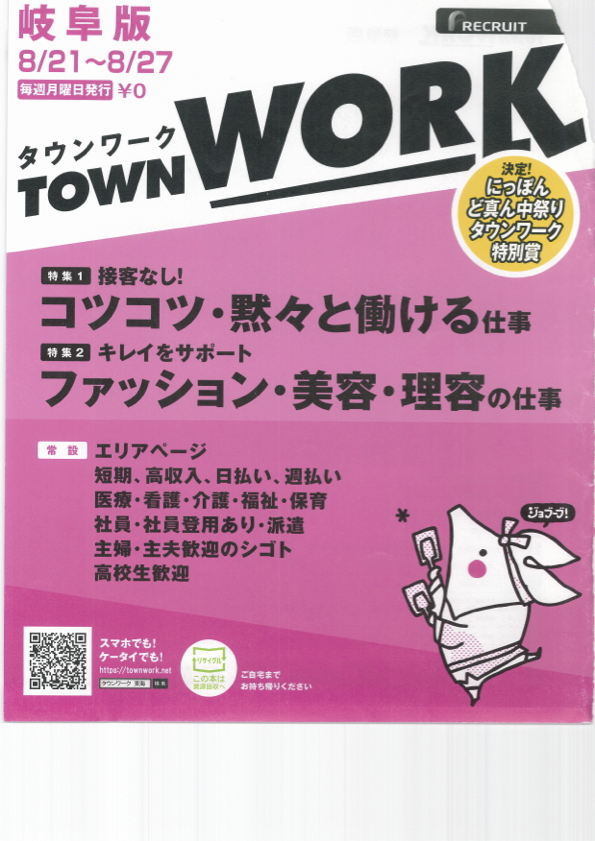
\includegraphics[scale=0.2]{tw7}
  \end{minipage}\\
  \begin{minipage}{0.4\linewidth}
    \centering
    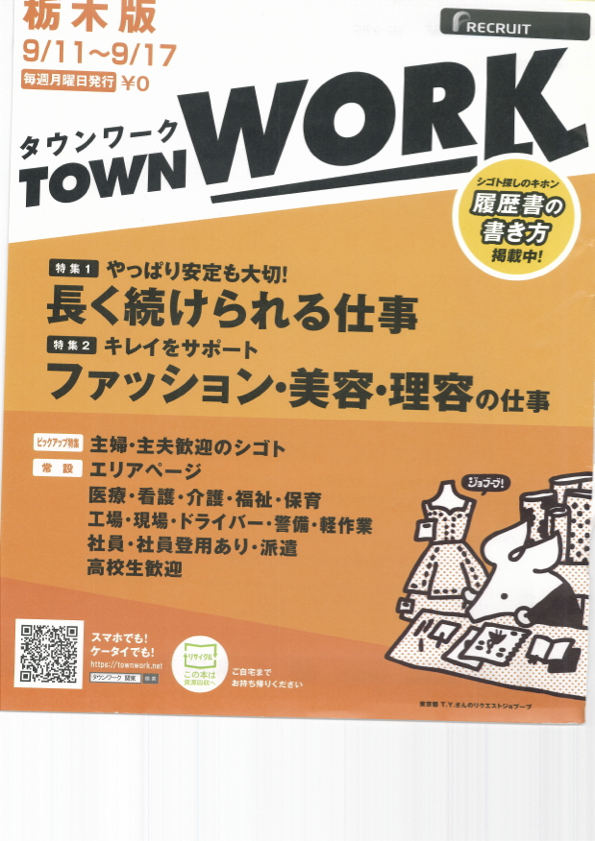
\includegraphics[scale=0.2]{tw8}
  \end{minipage}
  \begin{minipage}{0.4\linewidth}
    \centering
    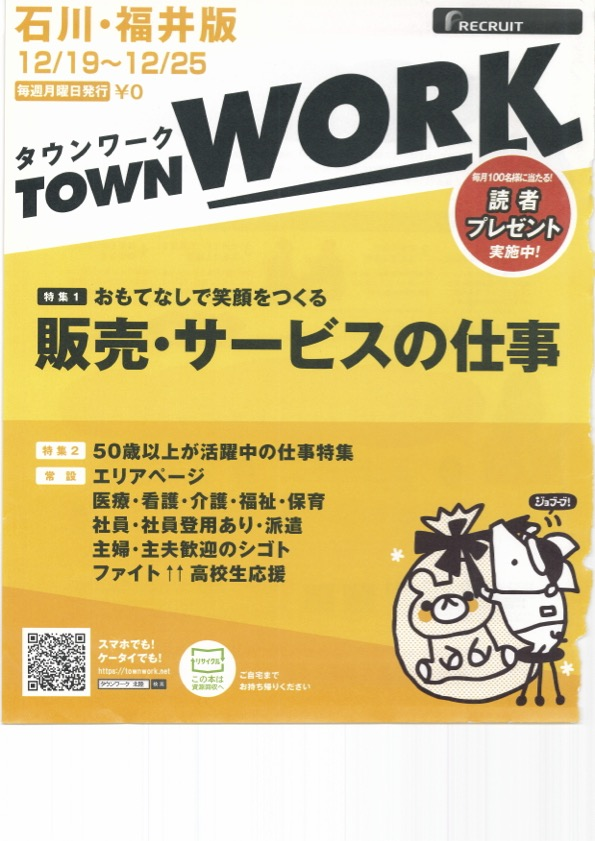
\includegraphics[scale=0.2]{tw9}
  \end{minipage}
  \begin{minipage}{0.4\linewidth}
    \centering
    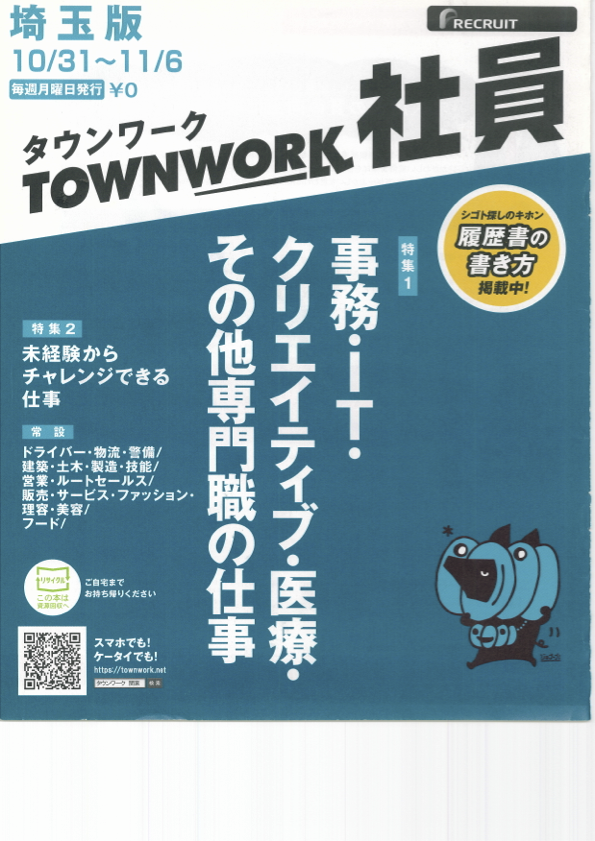
\includegraphics[scale=0.2]{tw10}
  \end{minipage}
  \begin{minipage}{0.4\linewidth}
    \centering
    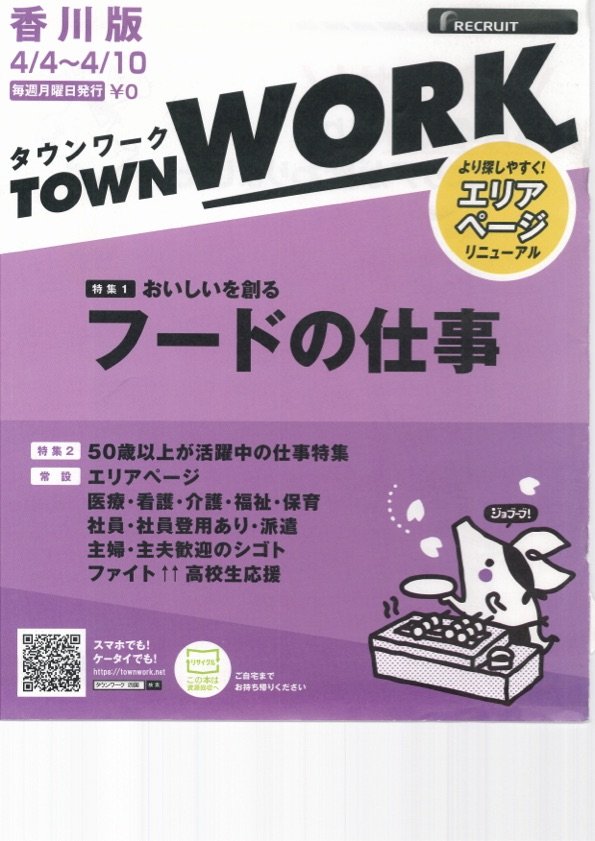
\includegraphics[scale=0.2]{tw11}
  \end{minipage}
  \caption{TownWorkの旅で手に入れた各地方の表紙一覧。}
  \label{CscDetaDphi-CSide}
\end{figure}

\newpage
\begin{figure}[htbp]
\vspace{-10mm}
    \centering
  \begin{minipage}{0.4\linewidth}
    \centering
    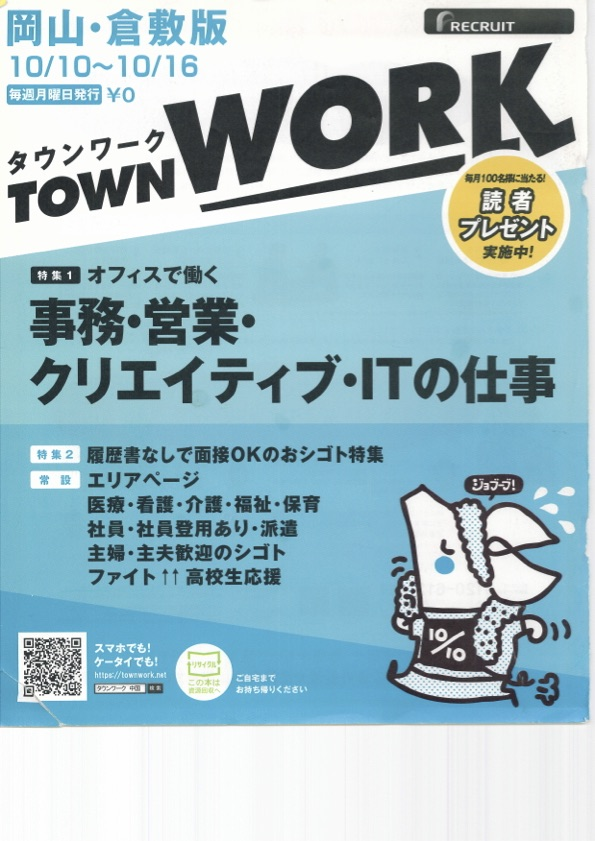
\includegraphics[scale=0.2]{tw12}
  \end{minipage}
  \begin{minipage}{0.4\linewidth}
    \centering
    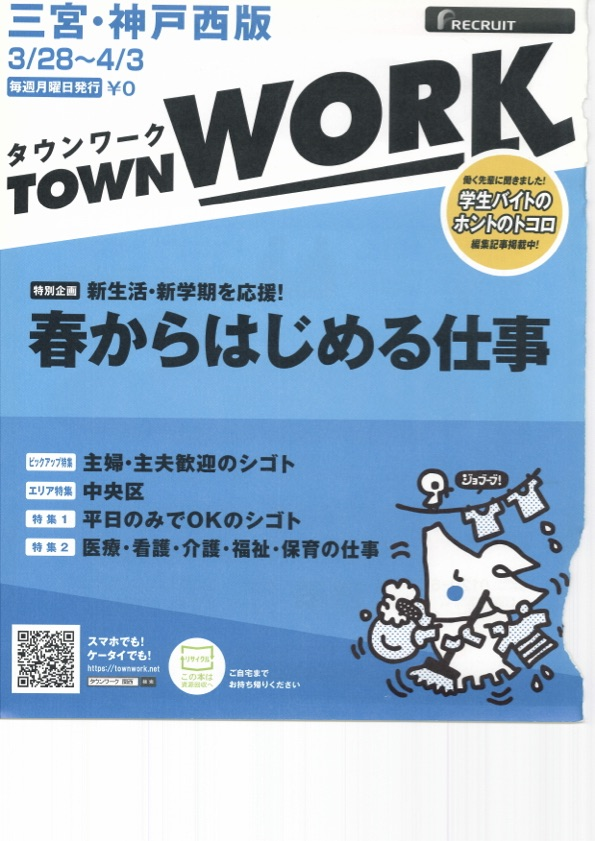
\includegraphics[scale=0.2]{tw13}
  \end{minipage}\\
  \begin{minipage}{0.4\linewidth}
    \centering
    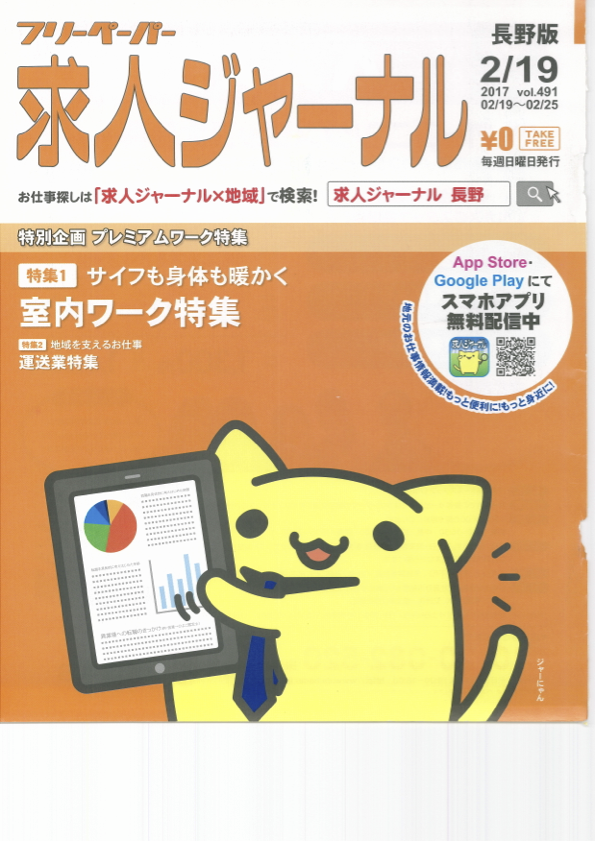
\includegraphics[scale=0.2]{tw14}
  \end{minipage}
  \begin{minipage}{0.4\linewidth}
    \centering
    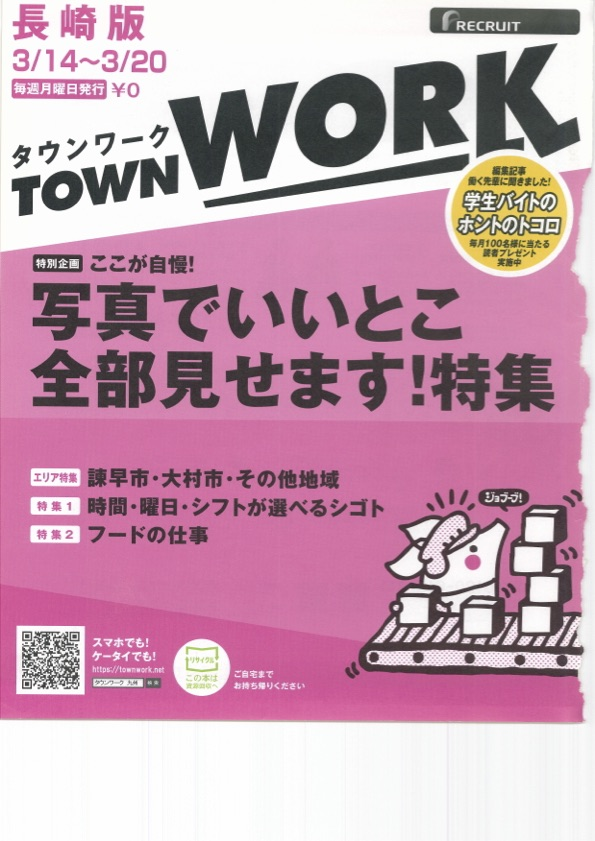
\includegraphics[scale=0.2]{tw15}
  \end{minipage}
  \begin{minipage}{0.4\linewidth}
    \centering
    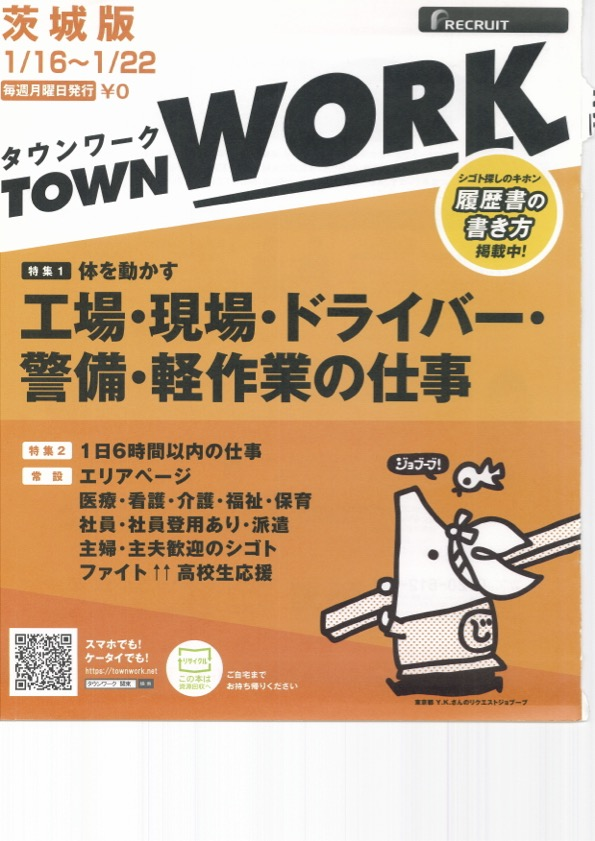
\includegraphics[scale=0.2]{tw16}
  \end{minipage}
  \begin{minipage}{0.4\linewidth}
    \centering
    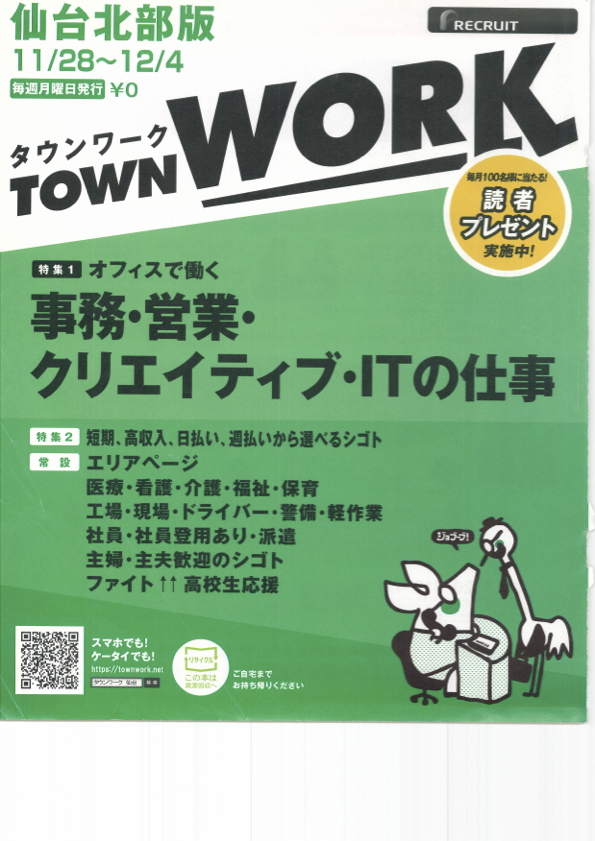
\includegraphics[scale=0.2]{tw17}
  \end{minipage}
  \caption{TownWorkの旅で手に入れた各地方の表紙一覧。}
  \label{CscDetaDphi-CSide}
\end{figure}

\newpage
\begin{figure}[htbp]
\vspace{-10mm}
    \centering
  \begin{minipage}{0.4\linewidth}
    \centering
    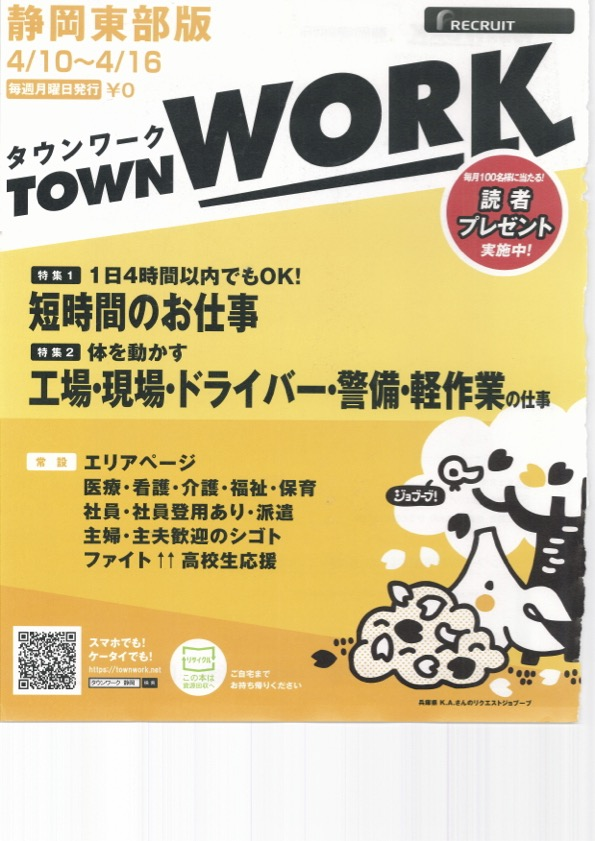
\includegraphics[scale=0.2]{tw18}
  \end{minipage}
  \begin{minipage}{0.4\linewidth}
    \centering
    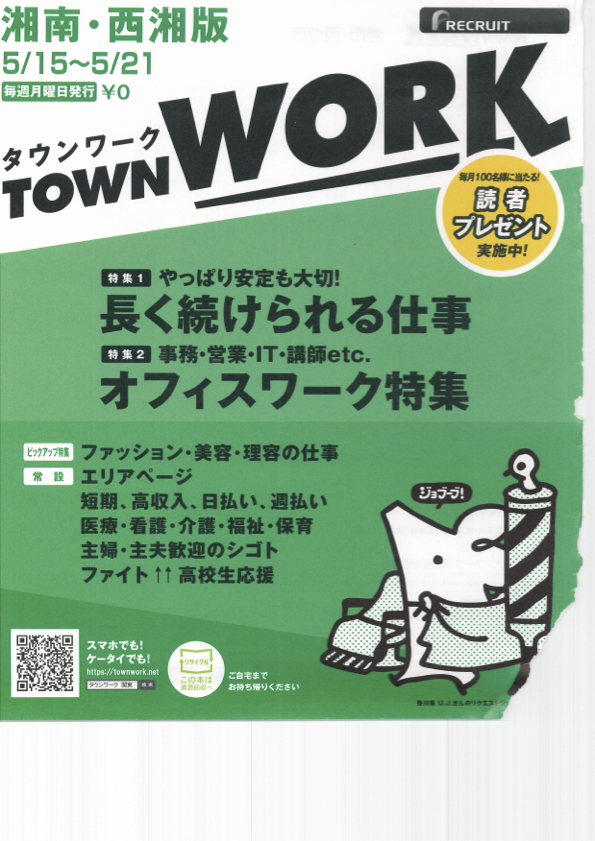
\includegraphics[scale=0.2]{tw19}
  \end{minipage}\\
  \begin{minipage}{0.4\linewidth}
    \centering
    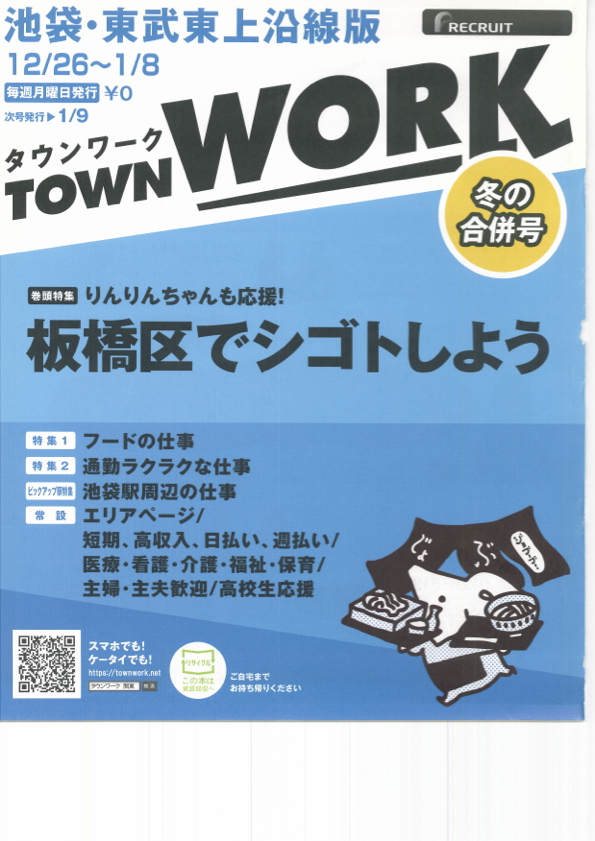
\includegraphics[scale=0.2]{tw20}
  \end{minipage}
  \begin{minipage}{0.4\linewidth}
    \centering
    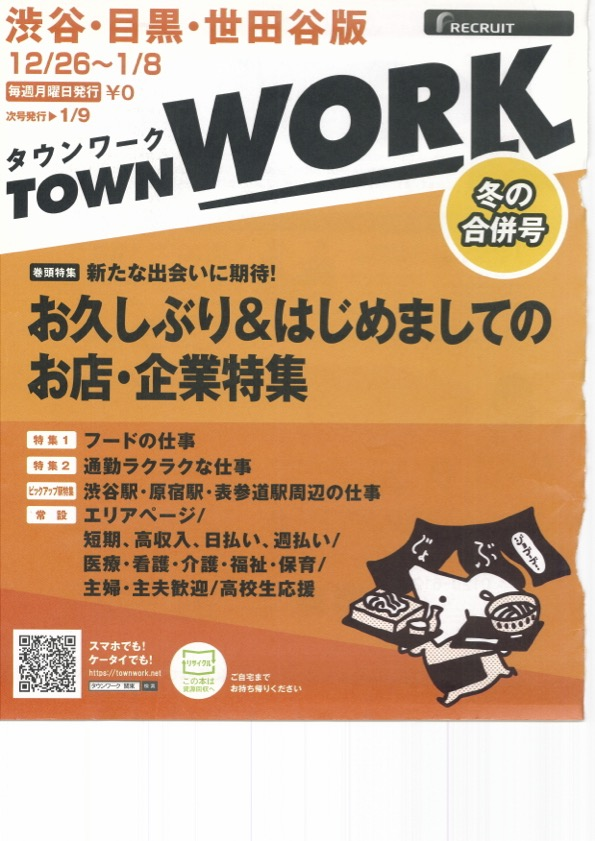
\includegraphics[scale=0.2]{tw21}
  \end{minipage}
  \begin{minipage}{0.4\linewidth}
    \centering
    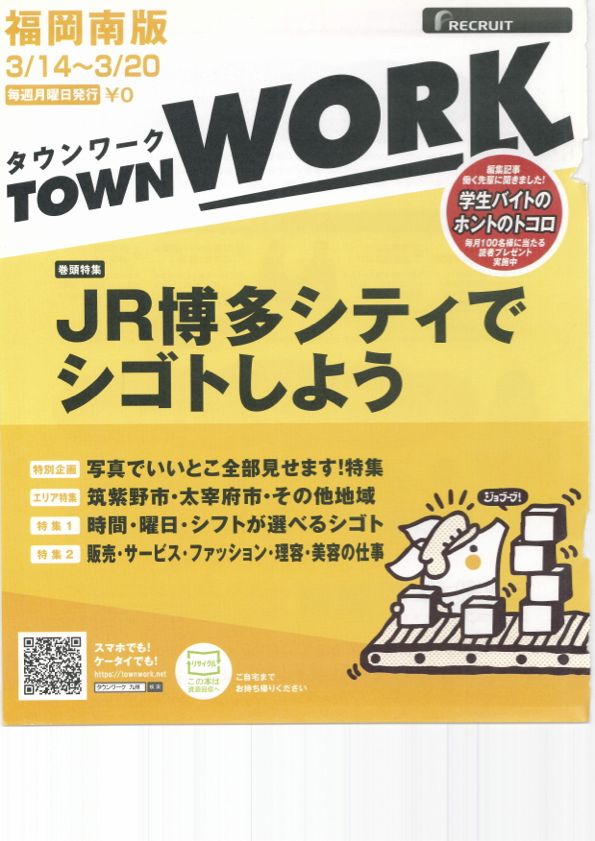
\includegraphics[scale=0.2]{tw22}
  \end{minipage}
  \caption{TownWorkの旅で手に入れた各地方の表紙一覧。}
  \label{CscDetaDphi-CSide}
\end{figure}

\newpage
\clearpage
%=========================%
\subsection{現在までに制覇された植民地}
%=========================%
以上の情報から、現在までに植民地とすることのできた県を示す。
ここで植民地とはタウンワーク情報を取得することのできた県であることを示しており、
色が着色されている部分が現在(2018年3月27日)までの植民地である。
また、これら新しく制覇された県を検出することのできるTownWorkの旅検出器板(TW-Board)
の開発も同時並行で行われた。
この新検出器板開発に際してCERNの各偉人たちの協力のもと設計・開発を行う予定であったが、
都合が合わず、そこで非言語大学独自の技術を用いた検出器板となった。

\begin{figure}
\centering
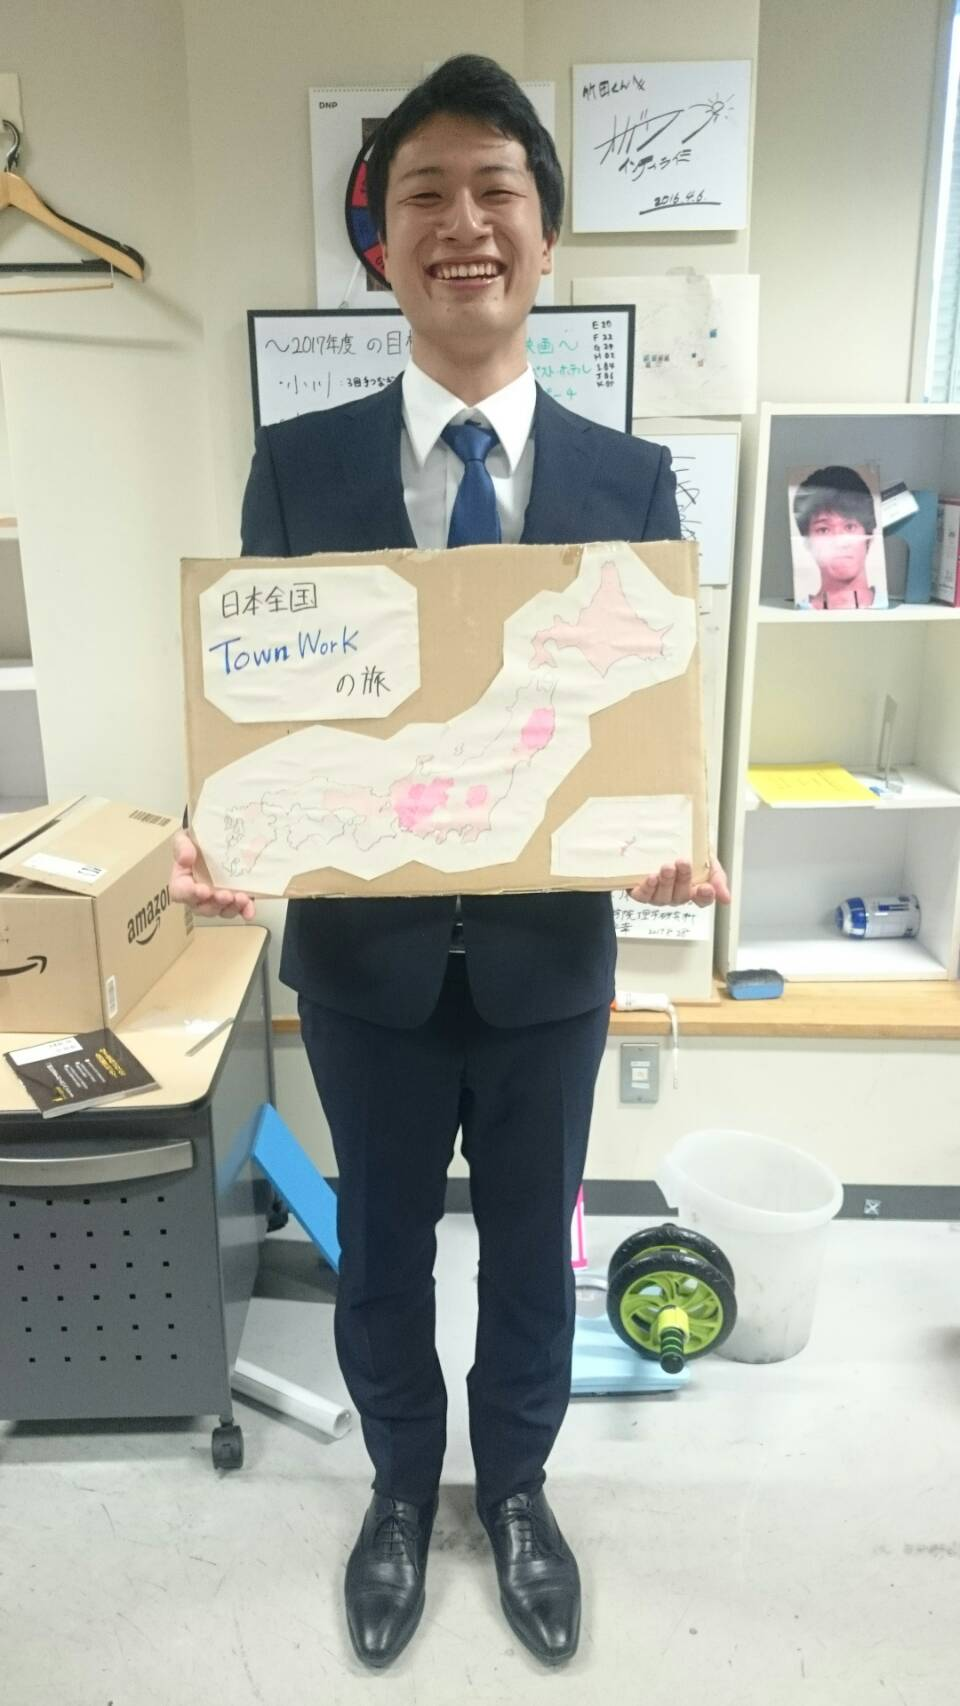
\includegraphics[scale=0.18]{TWBoard}
\caption{新検出器板を持ち、満面の笑みを浮かべるオマンガン伯爵。壁には山元大生、オガワインティライミのサイン、体重計等の懐かしのアイテムが転がっている。}
\label{oyayubi}
\end{figure}

\newpage
\clearpage
